\documentclass[default,pdf,colorBG,slideColor]{prosper}
\usepackage[T1]{fontenc}
\usepackage{epsfig}
\usepackage{pstricks}
\usepackage{graphicx}
\usepackage{listings}
\usepackage{xcolor}

\graphicspath{ {./fig/} {../fig/} }

\title{Flux Prototype Status}
\subtitle{{\small {\em prototype status}\\
LLNL-PRES-XXXXXX-DRAFT}}
\author{Jim Garlick}
\email{{\rm garlick@llnl.gov}}
\institution{Livermore Computing \\
             Lawrence Livermore National Laboratory}

\newcommand{\ngrm}{Flux}
\newcommand{\zMQ}{\O{}MQ}

% For listings:
\newcommand\Small{\fontsize{6}{6.2}\selectfont}
\newcommand\Smaller{\fontsize{5.5}{5.5}\selectfont}
\newcommand\realnumberstyle[1]{}
\makeatletter
\newcommand{\zebra}[2]{%
    {\realnumberstyle{#2}}%
    \begingroup
    \lst@basicstyle
    \ifodd\value{lstnumber}%
        \color{#1}%
        \rlap{\hspace*{\lst@numbersep}%
        \color@block{\linewidth}{\ht\strutbox}{\dp\strutbox}%
        }%
    \fi
    \endgroup
}
\makeatother

\slideCaption{\ngrm\ Progress Report, July. 16, 2014}

%\Logo(-1,-1){
\epsfig{file=graphic/iccd_logotrans.ps,scale=0.15}}


\begin{document}

% ==========================================================================
%\maketitle
% ==========================================================================

\begin{slide}{Flux Building Blocks}{\small
\begin{itemize}
  \item{\zMQ}
  \item{Comms Message Broker}
  \item{KVS}
\end{itemize}
}\end{slide}

% ==========================================================================
%\part{\zMQ}
% ==========================================================================
\begin{slide}{\zMQ}{\small
\begin{minipage}{0.50\textwidth}
\begin{itemize}
  \item{zguide.zeromq.org\\
        rfc.zeromq.org\\
        github.com/zeromq}
  \item{socket types:\\ req+rep, {\blue dealer+router}, {\blue pub+sub},
        push+pull}
  \item{endpoint types:\\
        {\tt tcp://{\em addr}:{\em port}}\\
        {\tt ipc://{\em path}}\\
        {\tt inproc://{\em name}}\\
        {\tt epgm://{\em iface};{\em addr}:{\em port}}}
 \end{itemize}
\end{minipage}
\begin{minipage}{0.50\textwidth}
\begin{itemize}
  \item{sockets can bind/connect multiple endpoints}
  \item{messages are atomic}
  \item{async I/O thread(s)}
  \item{curvecp/krb5}
  %\item{many language bindings}
  \item{C4.1 rfc.zeromq.org/spec:22}
\end{itemize}
\end{minipage}
}\end{slide}

\begin{slide}{\zMQ\ pub+sub}{\small
\begin{center}
  \includegraphics[scale=0.17]{zmq_pub_sub}
\end{center}
}\end{slide}

\begin{slide}{\zMQ\ dealer+router}{\small
\begin{center}
  \includegraphics[scale=0.20]{zmq_dealer_router}
\end{center}
}\end{slide}


% ==========================================================================
%\part{cmb}
% ==========================================================================

\begin{slide}{cmb - comms message broker}{\small
\begin{minipage}{0.50\textwidth}
\begin{itemize}
  \item{three overlay networks:\\
        - TBON for requests\\
        - ring for rank addr\\
        - bus for events}
  \item{comms modules:\\
        - message driven (CSP)\\
        - distributed services\\
        - dynamic loading}
  \item{ranked nodes\\
        {\em node} is a cmbd instance}
 \end{itemize}
\end{minipage}
\begin{minipage}{0.50\textwidth}
\begin{itemize}
  \item{master/slave architectures}
  \item{session heartbeat event\\
        - synchronized overhead}
  \item{data reduction}
  \item{reactor interface}
  \item{API socket for utilities}
  \item{utils: flux cmd [args]}
  \item{self-healing}
\end{itemize}
\end{minipage}
}\end{slide}

\begin{slide}{cmbd plumbing}{\small
\begin{center}
  \includegraphics[scale=0.20]{cmbd_sockets}
\end{center}
}\end{slide}

\begin{slide}{cmbd overlays}{\small
\begin{center}
  \includegraphics[scale=1.5]{B_Tree}
\end{center}
}\end{slide}

\begin{slide}{simplified example: echo server}
{\tiny\bf
\begin{lstlisting}[
 frame=shadowbox,
 rulesepcolor=\color{gray},
 numbers=left,
 numbersep=10pt,
 numberstyle=\tiny\zebra{gray!25},
 basicstyle=\Small\tt,
 ]
// comms module request callback
void echo_cb (flux_t h, int typemask, zmsg_t **zmsg, void *arg)
{
    JSON request  = NULL;
    if (cmb_msg_decode (*zmsg, NULL, &request) >= 0) {
        int i, repeat;
        const char *s;

        /* 'string' to echo is required. */
        if (!Jget_str (request, "string", &s)) {
            flux_respond__errnum (h, zmsg, EINVAL);
            goto out;
	}
        /* 'repeat' is optional */
        if (!Jget_int (request, "repeat", &repeat))
            repeat = 1;
        for (i = 0; i < repeat; i++) {
            zmsg_t *z = zmsg_dup (*zmsg);
            JSON resp = json_echo (s, p->conf->rank);
            flux_respond (h, &z, resp);
            Jput (resp);
        }
    }
out:
    Jput (request);
    zmsg_destroy (zmsg);
}
\end{lstlisting}
} \end{slide}

\begin{slide}{simplified example: echo client}
\vspace{-0.3in}
{\tiny\bf
\begin{lstlisting}[
 frame=shadowbox,
 rulesepcolor=\color{gray},
 numbers=left,
 numbersep=10pt,
 numberstyle=\tiny\zebra{gray!25},
 basicstyle=\Smaller\tt,
 ]
int main (int ac, char *av[])
{
    flux_t h;
    JSON request;
    int id, i, ncopies = 1;

    if (!(h = cmb_init ()))
	fatal ("failed to open Flux handle: %s\n", strerror (errno));

    if (ac > 3)
        ncopies = atoi (av[2]);

    request = Jnew ();
    Jadd_str (request, "string", av[1]);
    Jadd_int (request, "repeat", ncopies);
    
    if (flux_request_send (h, request, "echo") < 0)
        fatal ("flux_request_send: %s\n", strerror (errno));

    for (i = 0; i < ncopies; i++) {
        JSON response;
        const char *s;

        if (flux_response_recv (h, &response, NULL, false) < 0)
            fatal ("flux_response_recv: %s\n", strerror (errno));

        Jget_str (response, "string", &s);
        Jget_int (response, "id", &id);
        printf ("got reply %d from %d: %s\n", i+1, id, s);
        Jput (response);
    }
    flux_handle_destroy (&h);
    return (0);
}
\end{lstlisting}
} \end{slide}


% ==========================================================================
%\part{KVS}
% ==========================================================================

\begin{slide}{KVS}{\small
\begin{minipage}{0.50\textwidth}
\begin{itemize}
  \item{master/slave architecture\\
        - master rank=0 \\
        - slaves rank>0 }
  \item{primary operations:\\
        {\tt kvs\_get()}\\
        {\tt kvs\_put()}\\
        {\tt kvs\_commit()}\\
        {\tt kvs\_watch()}\\
        {\tt kvs\_fence()}}
  \item{in-memory only\\
        (no persistence yet)}
 \end{itemize}
\end{minipage}
\begin{minipage}{0.50\textwidth}
\begin{itemize}
  \item{object store\\
        - hash by value\\
        - hierarchical namespace}
  \item{caching slaves\\
        - eventually consistent\\
        - temporal cache\\
        - recursive pull from parent}
  \item{cache update:\\
        - mcast new root SHA1}
\end{itemize}
\end{minipage}
}\end{slide}

\begin{slide}{kvs get a.b.c}{\small
\begin{minipage}{0.50\textwidth}
\begin{enumerate}
\item{load root from {\tt 1c002dde}, find {\tt a} is at
{\tt 3f2243ef}.}
\item{load {\tt a} from {\tt 3f2243ef}, find {\tt b} is at
{\tt 023e9b2d}.}
\item{load {\tt b} from {\tt 023e9b2d}, find {\tt c} is at
{\tt 7ff234a8}.}
\item{load {\tt c} from {\tt 7ff234a8}, and return it (42).}
\end{enumerate}
\end{minipage}
\begin{minipage}[t]{0.50\textwidth}
\begin{center}
  \includegraphics[scale=0.20]{kvs_update_1}
\end{center}
\end{minipage}
}\end{slide}

\begin{slide}{kvs put a.b.c=43}{\small
\begin{minipage}{0.50\textwidth}
\begin{enumerate}
\item{store 43 to {\tt 62302aff}.}
\item{update {\tt b} to associate {\tt c} with {\tt 62302aff}, and store {\tt b} to {\tt 8fe9b2c3}.}
\item{update {\tt a} to associate {\tt b} with {\tt 8fe9b2c3}, and store {\tt a} to {\tt aacc76b4}.}
\item{update root to associate {\tt a} with {\tt aacc76b4}, and store root to {\tt 033fbe92}.}
\end{enumerate}
\end{minipage}
\begin{minipage}[t]{0.50\textwidth}
\begin{center}
  \includegraphics[scale=0.20]{kvs_update_2}
\end{center}
\end{minipage}
}\end{slide}

\begin{slide}{finalize kvs commit}{\small
\begin{minipage}{0.50\textwidth}
\begin{enumerate}
\item{new root reference is {\tt 033fbe92}.}
\end{enumerate}
\end{minipage}
\begin{minipage}[t]{0.50\textwidth}
\begin{center}
  \includegraphics[scale=0.20]{kvs_update_3}
\end{center}
\end{minipage}
}\end{slide}

% ==========================================================================
\part{extra slides}
% ==========================================================================

\begin{slide}{self-healing example}{\tiny
\begin{verbatim}
$ salloc -N 8
$ scripts/launch -c trinary
$ flux topo -H | dot -Tpng | display
\end{verbatim}
\begin{center}
  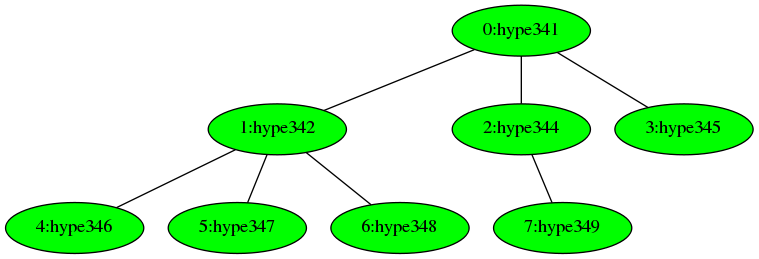
\includegraphics[scale=1]{8tri-ok}
\end{center}
}\end{slide}

\begin{slide}{self-healing example}{\tiny
\begin{verbatim}
$ flux peer --rank 1 panic
$ flux up
ok:     [0,2-7]
slow:
fail:   1
unknown:
$ flux topo -H | dot -Tpng | display
\end{verbatim}
\begin{center}
  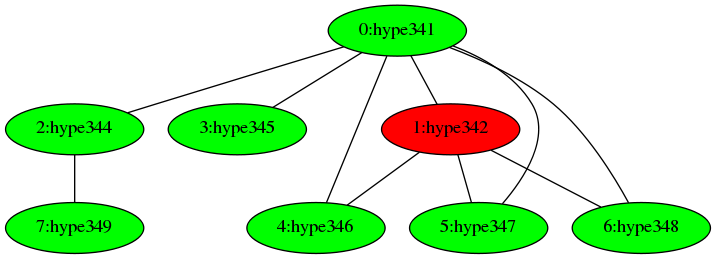
\includegraphics[scale=1]{8tri-fail}
\end{center}
}\end{slide}


\end{document}
